\setlength{\columnsep}{3pt}
\begin{flushleft}
	\bigskip
	There are 2 major types of editors in Linux:
	\begin{itemize}
		\item \textbf{Grahpical editor}
		\begin{itemize}
			\item \textbf{gedit}: 	Gedit application is a full-featured text editor.
			\begin{tcolorbox}[breakable,notitle,boxrule=0pt,colback=pink,colframe=pink]
				\color{black}
				\fontdimen2\font=1em
				Syntax: gedit filename
				\fontdimen2\font=4pt
			\end{tcolorbox}
			Eg:
			\begin{figure}[h!]
				\centering
				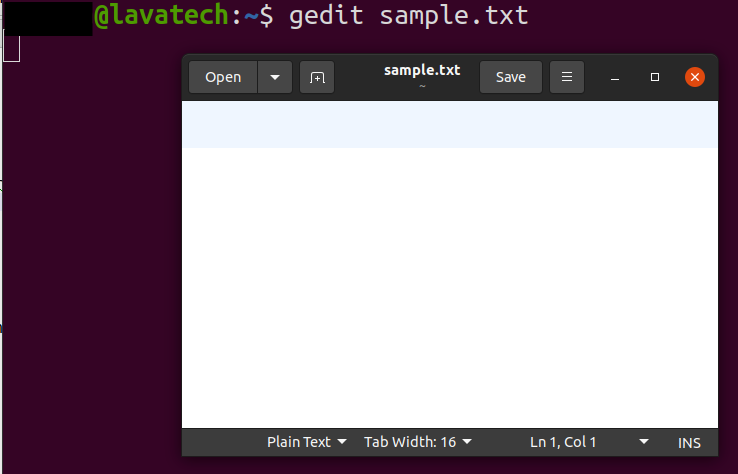
\includegraphics[scale=0.4]{content/chapter3/images/gedit.png}
				\caption{Sample output}
				\label{fig:cal32}
			\end{figure}
			
		\end{itemize}
		\item \textbf{Text-based editor}
		\begin{itemize}
			\item \textbf{vi or vim}:  Text based editor used in Linux and Mac OS. Let's see more on this.
		\end{itemize}
	\end{itemize}
\end{flushleft}

\newpage





